\documentclass[a4paper, norsk, twoside, 10pt]{article}
\usepackage[utf8]{inputenc}
\usepackage[a4]{}
\usepackage[norsk]{babel}
\usepackage{amsmath}
\usepackage{amsthm}
\usepackage{amssymb}
\usepackage{color}
\usepackage{listings}
\usepackage{graphicx}
\usepackage{epsfig}
\usepackage{float}
\usepackage{fancyhdr}

\author{Elsie Mestl}
\date{\today}
\title{Oblig 2 \\ matinf1100 - Modelering og beregninger}


\pagestyle{fancy}
\lhead{Oblig 2. \quad matinf1100-Modelering og beregninger}
\rhead{Elsie Mestl}

\begin{document}

\maketitle

\section*{Oppgave 1}
\lstinputlisting[language=Python]{oppgave1.py}

\begin{figure}[H]
  \centering
  \textbf{Plot}\par\medskip
  \caption{Top grafen viser akselerasjonen per tid. Den nedre viser avstand fra start per tid.}
  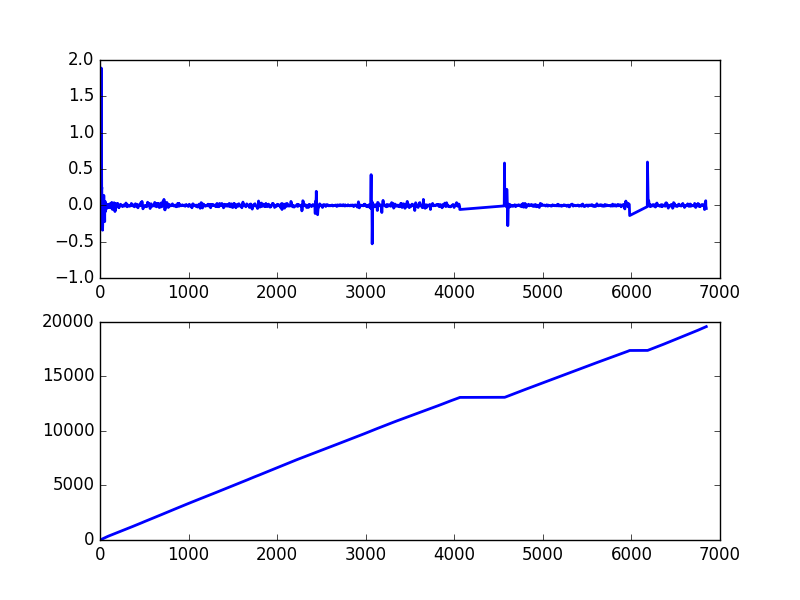
\includegraphics[width = \textwidth ]{opgv1.png}
\end{figure}

\section*{Oppgave 2}
\subsection*{a)}
\begin{align*}
  &x' + x^2 = 1 && x(0) = 0 \\
  \intertext{Hvor x er en funksjon av t og skrives x(t)}
  x'(t)& = 1 - x^2(t) \\
  \frac{x'(t)}{1-x^2(t)} & = 1 \\
  \int \frac{x'(t)}{1-x^2(t)} dt &= \int 1 dt &&\text{substituer for }x = x(t) \\
  \int \frac{1}{1- x^2} dx &= \int\frac{1}{(1-x)(1+x)} dx= \int \frac{1}{2(1-x)}dx + \int \frac{1}{2(1+x)} dx \\ &= \frac{1}{2}\ln(1 +x) + C_1 - \frac{1}{2}\ln(1-x) + C_2 = t +C_3\\
  \ln\left(\frac{1+x}{1-x}\right) &= 2t + C\\
  \frac{1+x}{1-x} &=  e^{2t+C}  \\
  1 + x &= e^{2t + C} - xe^{2t + C} \implies x(e^{2t + C} +1) =  e^{2t + C} -1
  \ \\
  x(t) &= x= \frac{e^{2t}D -1}{e^{2t}D + 1} &&\text{hvor $D = e^C$}
  \intertext{for den spesielle løsningen har vi}
  x(0) &= \frac{D -1}{D +1} = 0  \implies D-1 = 0 \implies D = 1 \\
  x(t) &= \frac{e^{2t} - 1}{e^{2t} +1}
\end{align*}


\subsection*{b, c)}
\lstinputlisting[language=Python]{oppgave2b.py}

\begin{figure}[H]
  \centering
  \textbf{Plot}\par\medskip
  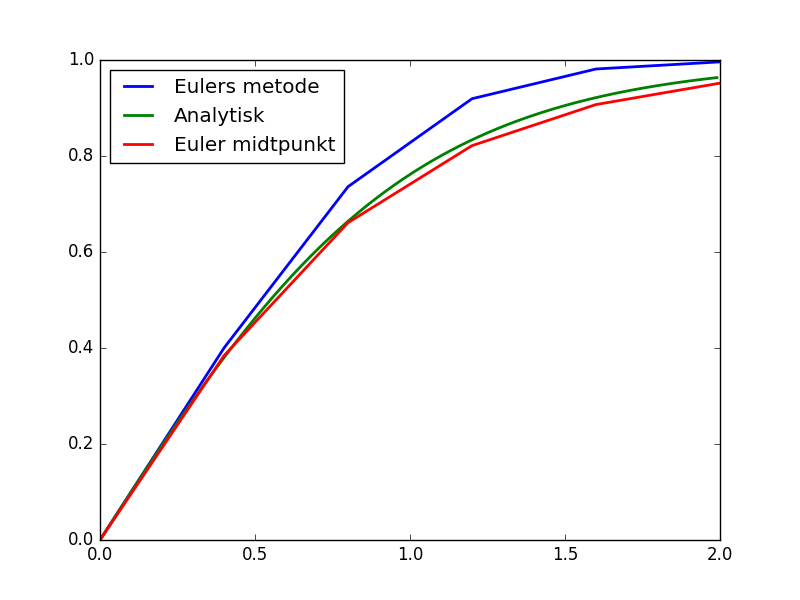
\includegraphics[width = \textwidth ]{opgv2.png}
\end{figure}



\subsection*{d)}
Fra (1) har vi at $x' = 1 - x^2$, altså at $x'(t) = 1- x^2(t)$. Hvis $0 \leq x(t^*) < 1$ har vi at $|x(t^*)| < 1 \implies x^2(t^*) < 1$. Setter vi inn i likningen får vi at $x'(t) > 0$. Siden den deriverte er positiv vil grafen, $x(t^*)$, være voksende. \\

Hvis $x(t^*) > 1 $ eller $x(t^*) = 1$ får vi etter samme argumentasjon respektivt $x'(t^*) < 0$ og $x'(t^*) = 0$ som vil si at $x(t^*)$ respektivt minker og er konstant.


\subsection*{e)}
Fra a) har vi at den gennerelle løsningen til difflinkningen er
\[  x(t) =  \frac{e^{2t} -1}{e^{2t} + 1} \]
Setter vi  inn i linkning (1) får vi.
\[x'(t) = 1 - \left(\frac{e^{2t} -1}{e^{2t} + 1}\right)^2 \]
For at x skal være voksende må $\frac{e^{2t} -1}{e^{2t} + 1} \leq 1$ for $t\geq0$. Og siden $e^{2t}$ alltid er positiv og større eller lik 1 for $t \geq 0$ har vi at $e^{2t} -1 \leq e^{2t} + 1 \implies \frac{e^{2t} -1}{e^{2t} + 1} \leq 1$  for $t \geq 1$. Og vi har at $x(t)$ er voksende for alle $t$ større eller lik 0.
\end{document}
